\chapter{Background}

This chapter gives an overview of SCION, briefly describing the core concepts, the network structure and essential components, all required to understand the context of this thesis. For an in-depth understanding please refer to \cite{scion_book}.

\section{SCION - A Future Internet Architecture}

\fnurl{SCION}{https://github.com/netsec-ethz/scion} is a future Internet architecture with the goal to offer a "highly available", secure and transparent "point-to-point packet delivery" infrastructure. \cite[Page~17]{scion_book} SCION tackles problems with respect to political and economical issues, today's internet suffers from. These properties can even be fulfilled in presence of malicious network members.

To realize above ambitions SCION makes use of sophisticated techniques. The most important of these concepts are described below:

\begin{figure}
	\centering
	\centerline{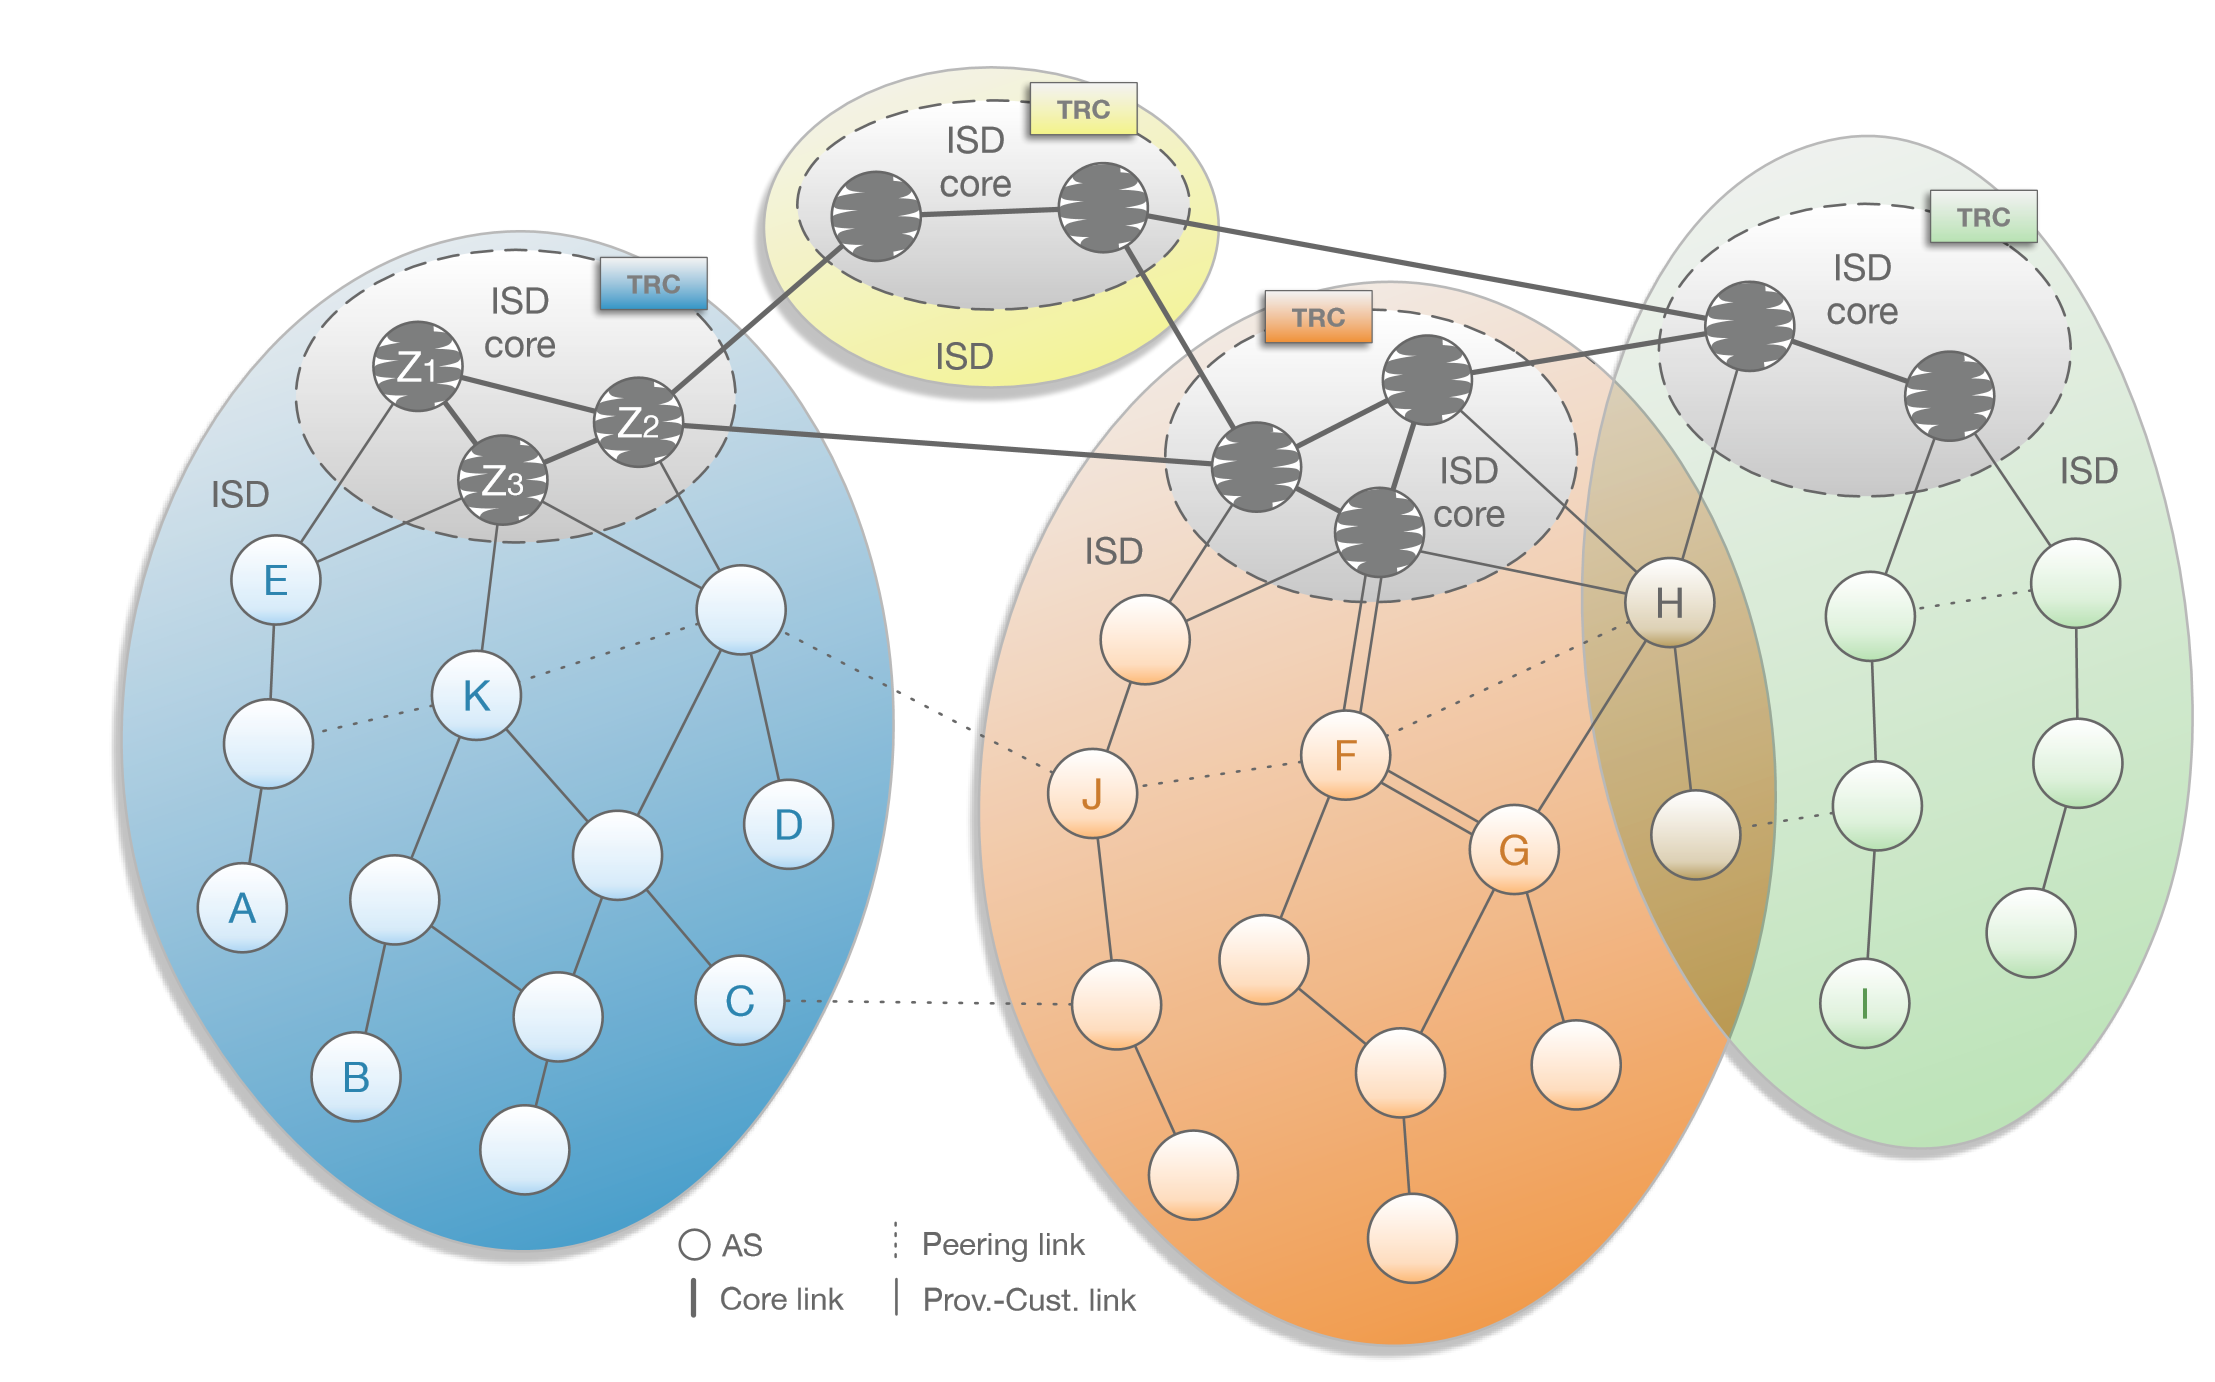
\includegraphics[width=\linewidth]{scion_overview.png}}
	\captionof{figure}{Schematic overview of a SCION network consisting of four ISDs \cite{scion_book}}
	\label{back:overview}
\end{figure}


\subsection{Network Structure}
\label{back:network_structure}
SCION organizes Autonomous Systems (ASes) into entities called Isolation Domains (ISDs). A selection of ASes in an ISD are designated 
core ASes responsible for administering the ISD. For example, the core ASes  negotiate the roots of trust used for authentication. An AS can join an ISD by connecting to an AS that already is a member of the ISD. Joining an ISD implies agreeing to the policies governing the ISD. \cite[Chapter~2]{scion_book}

\subsection{Isolation}
SCION divides the network into isolated entities called Isolation Domains and lets these ISDs manage their own part of the network, including the election of authorities and properties like routing policies and key agreement. This enables SCION to divide the control plane in a way such that one ISD is not influenced by changes in any other ISD. As an example, this mitigates outages (therefore increasing availability as desired) caused by accidentally or even maliciously misconfigured ASes, which make BGP announcements for addresses they have no control over. whereas In today's Internet, potentially every host could be affected. \cite[Chapter~3]{scion_book} Figure \ref{back:overview} shows a network with four ISDs, each consisting of multiple ASes.
	
\subsection{Path Selection}
SCION allows each host to control routes for outgoing and incoming packages. For each AS different paths, so called up-paths, are constructed using \textit{Path Construction Beacons} (PCBs). These PCBs reflect the constraints imposed by the ISD routing policy. ASes then announce over which of these paths they want to be reached. This technique, amongst other advantages, makes it possible to deploy effective mechanisms against Denial of Service attacks. Additionally, SCION offers a secure way of revoking failed paths and paths that do not conform to the route policy any more. \cite[Chapters~7, 10]{scion_book}
	
	\begin{figure}
		\centering
		\centerline{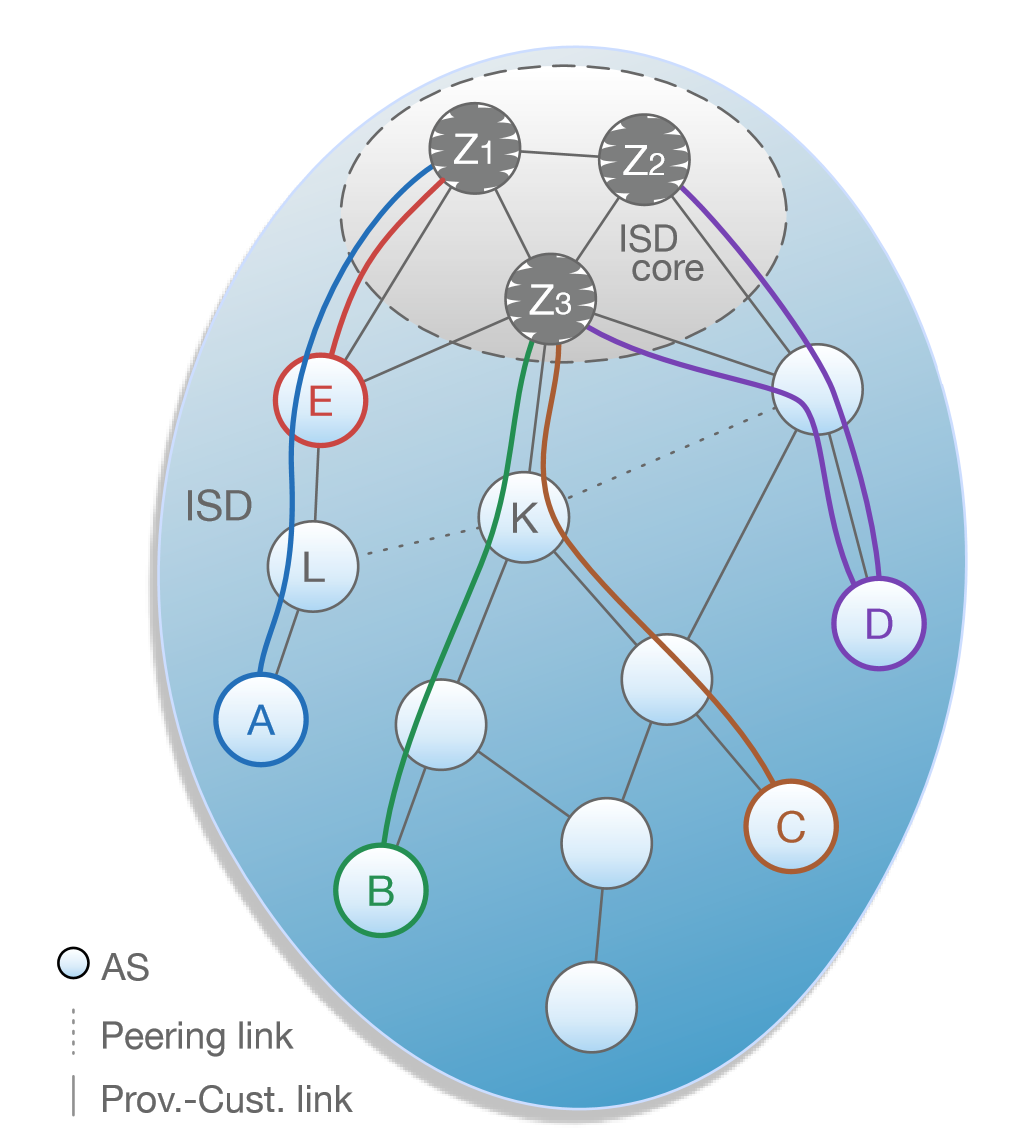
\includegraphics[height=8cm]{isd_paths.png}}
		\captionof{figure}{ISD with path segments for ASes A, B,C, D, and E \cite{scion_book}}
		\label{back:paths}
	\end{figure}

\subsection{Scalability}
The controlled path selection approach outlined above ensures great scalability, as opposed to source-based routing where every host needs to know the entire network topology. At the same time, the freedom of path selection is preserved. Furthermore, since routes are pre-determined, all the forwarding information is encoded in the package itself. This renders badly scaling routing and forwarding tables obsolete, all to the benefit of increased scalability. \cite{scion_book}


\section{SCION Architecture}

Following, important components of the SCION architecture are described. All the information is taken from \cite{scion_book}.
 
\subsection{Border Routers}
Border routers are responsible for inter-AS communication. They carry out packet forwarding based on the pre-determined path, encoded in each packet. Border routers work efficiently since the costly look up in a forwarding table is omitted.

\subsection{Beacon Servers}
The main function of the Beacon Server is to process path construction beacons (PCBs). The mechanism starts with a core AS generating initial PCBs and distributing them over the network. Beacon servers of non-core ASes upon receive propagate the PCBs down to their child ASes, such that the whole network is flooded. Through these beacons, ASes learn paths on which they can reach the ISD core. The AS then selects a subset of these paths and registers them using its Path server.

\subsection{Path Servers}
After processing PCBs, an AS registers at its local path server down-paths over which it wants to be reachable. This information is then used by other ASes to determine routes to that AS.

In reverse, the path server also functions as look up service via which an AS can retrieve path segments to reach another AS. When queried for an AS, the path server returns the paths available to reach the desired AS.

\subsection{Certificate Servers}
Local certificate servers manage and cache certificates of all members inside their AS, as well as the certificate issued by the ISD core to be used by the AS itself. For example, certificate servers support path servers by validating PCBs. \cite[Chapter~2]{scion_book}

A certificate server in the ISD core manages all certificates it handed out to ASes in its ISD and provides a validation service ASes can query.

\subsection{Name Servers}
Similar to the DNS system currently used in the Internet, name serves perform the translation from human-friendly names to addresses understood by SCION infrastructure. The path server is then queried to obtain end-to-end paths reaching the resolved address. \cite[Chapter~2]{scion_book} 


\section{SCION AS Management Framework}
\label{back:lmi}

For easy deployment and maintenance, SCION offers the SCION AS Management Framework which provides an intuitive web interface for deploying and managing ASes. The framework consists of a \lmi per AS and a global coordinator, the \lcs. This framework facilitates inter-AS communication by relaying connection requests between ASes. In Section \ref{back:network_structure} we explained how an AS can join an ISD by connecting to an AS that already is in said ISD. Such ISD join requests, for example, are handled by the framework. Figure \ref{back:deployment} shows three deployed ASes connected through the SCION AS Management Framework.

The following sections describe the two components of the framework in more detail.

\begin{figure}
	\centering
	\centerline{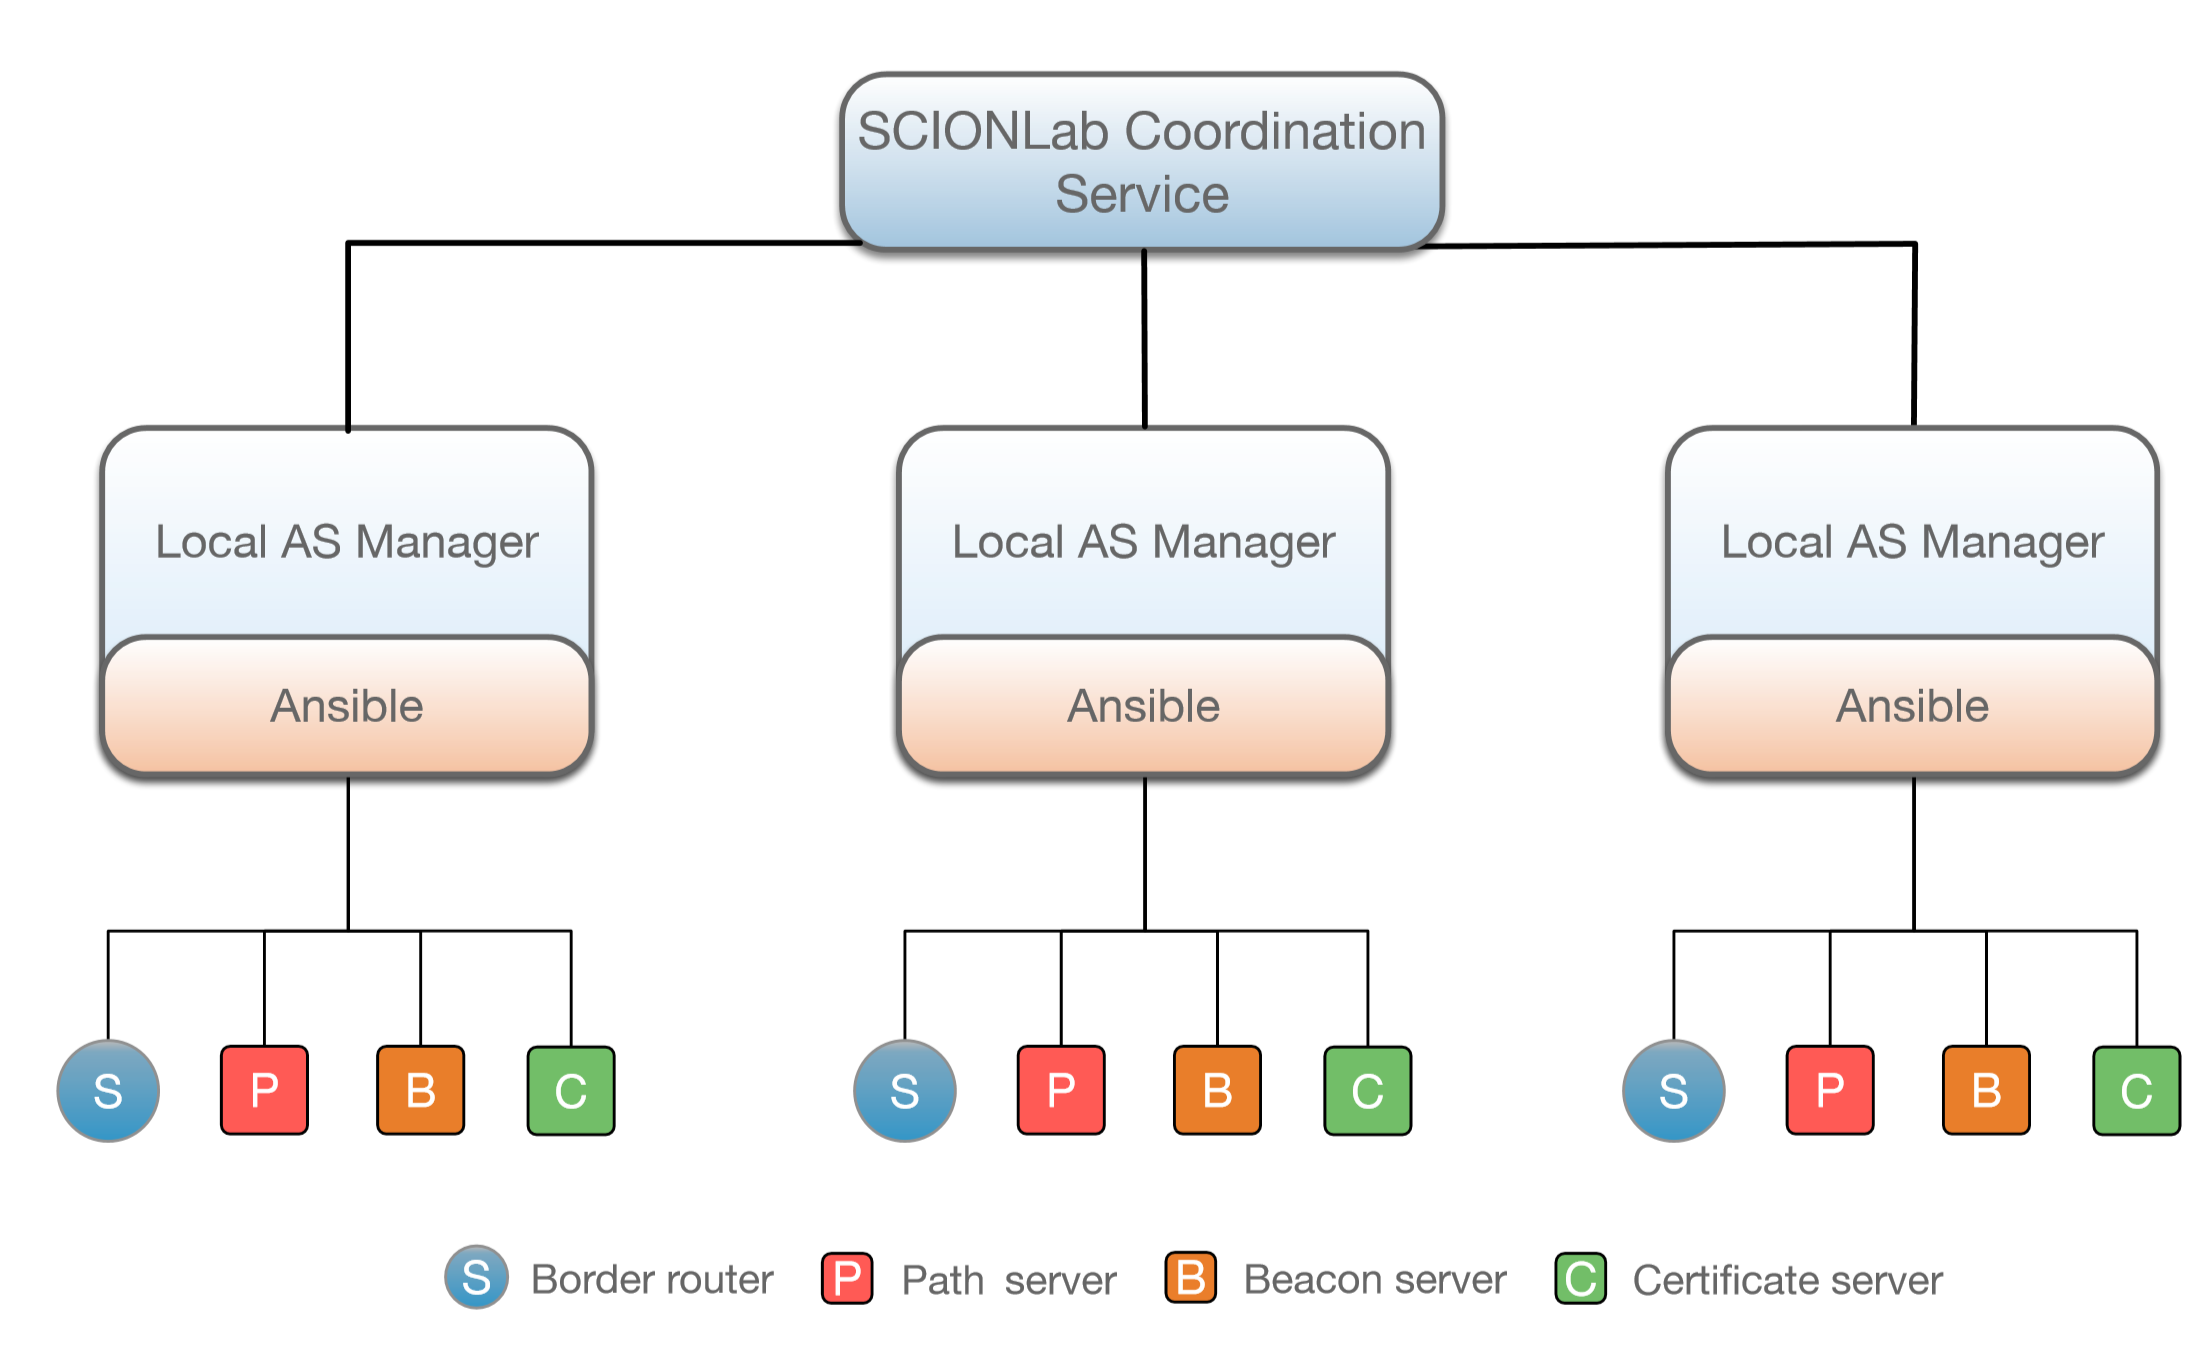
\includegraphics[width=\linewidth]{scion_deployment.png}}
	\captionof{figure}{Overview of deployment architecture showing the role of \lcs as mediator \cite{scion_book}}
	\label{back:deployment}
\end{figure}

\subsection{Local Management Service}

The \fnurl{\lmi}{https://github.com/netsec-ethz/scion-web} is the local component of the SCION AS Management Framework. It's run by the authority managing the AS, used to monitor and configure that AS. It offers a web interface through which, amongst other functionality, administrators can make connection requests to other ASes they wish to connect to. These requests, containing all the necessary data to set up a new link between the initiator and the remote AS, are then relayed via \lcs to the recipient AS. \cite[Chapter~10]{scion_book} In a similar fashion join requests for integrating an AS into an ISD can be issued using the \lmi. Other functionality involves generating the AS topology and the configurations to be deployed onto local servers.

Figure \ref{back:scionweb} shows the \lmi interface presented when making a connection request.

\begin{figure}
	\centering
	\centerline{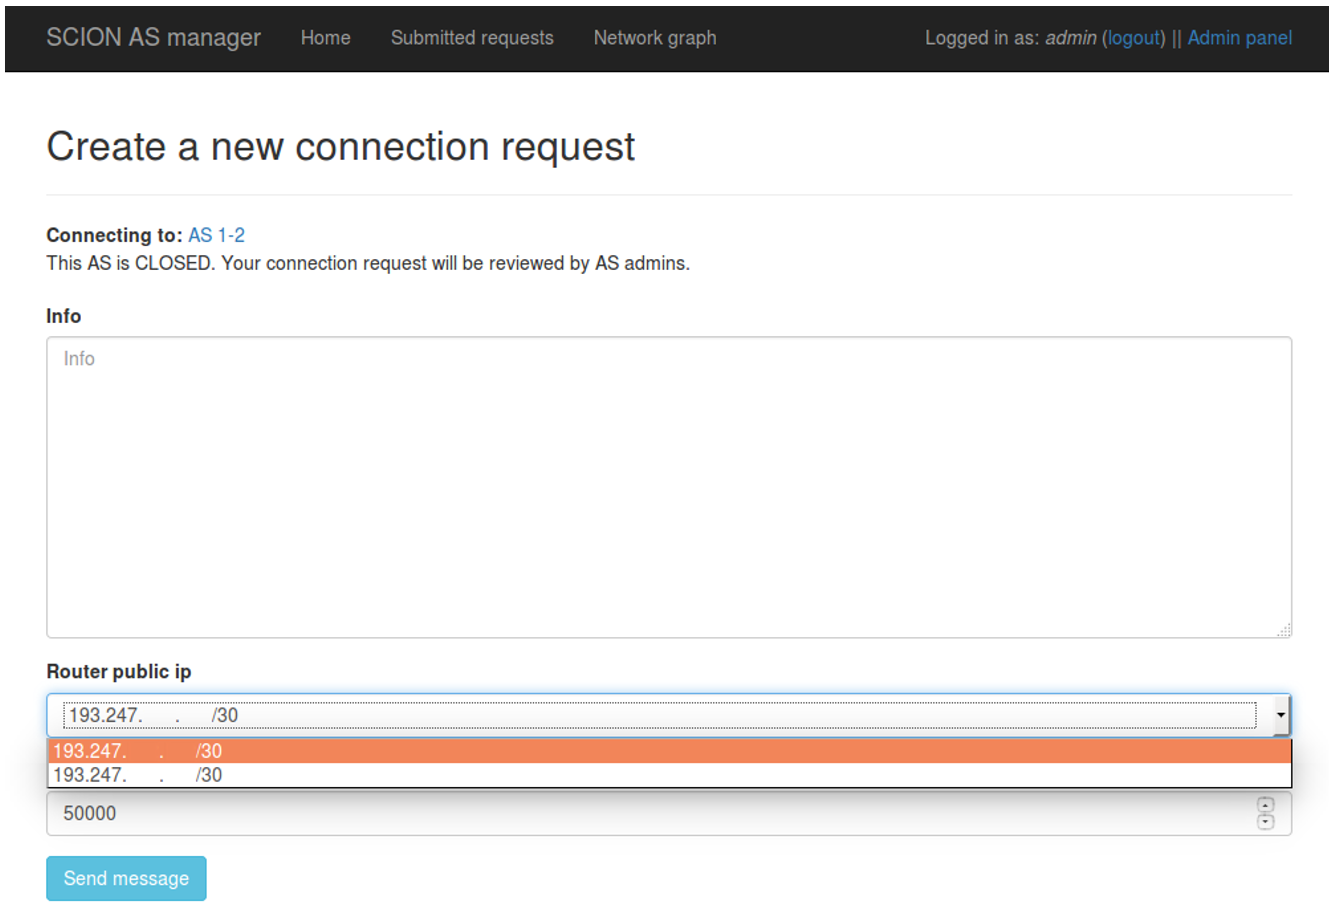
\includegraphics[width=\linewidth]{scionweb.png}}
	\captionof{figure}{\lmi used to make a connection request \cite{wirz}}
	\label{back:scionweb}
\end{figure}

\subsection{SCIONLab Coordination Service}
\label{back_scion_coord}

\fnurl{\lcs}{https://github.com/netsec-ethz/scion-coord} serves two purposes. For one it is part of the SCION AS Management Framework where it serves as a mediator between different \lmi instances. It provides information about available ISDs and ASes making it easy for new ASes to be created and connected to the SCION network. \lcs in the role of a mediator is not required by SCION. It's merely a tool to facilitate the deployment process in the early stages of adoption. Later, inter-AS connections will be negotiated between the involved parties directly. \cite[Chapter~10]{scion_book}

\lcs's second responsibility is the support of the \lee which lets interested organisations and institutions experiment with the unique capabilities of SCION. More detail about \lee and the role \lcs takes in it is available in Section \ref{back:scionlab}.

\section{SCIONLab Experimentation Environment}
\label{back:scionlab}

The \lee is a project started with the goal to provide a unique testbed environment, enabling researches to experiment with SCION and the features it offers. At the same time, it allows the SCION network to naturally grow by opening up the infrastructure. In SCIONLab, participants join by deploying their own ASes in the SCION network and then connecting to other SCIONLab ASes. Hence, SCIONLab forms a subset of the entirety of ASes deployed in the SCION network. Participants become an integral part of the network, actively partaking in routing. This allows researchers to conduct highly realistic experiments, not possible with other popular testbed environments. \cite[Chapter~10]{scion_book}

SCIONLab builds on the foundation of SCION AS Management Framework. It uses the same tools to offer a clean, easy-to-use way of joining the SCIONLab network.
As an example, \lcs facilitates the deployment of SCIONLab ASes for interested parties. It is envisioned to offer built in user administration capabilities, where users can register accounts and download SCIONLab configurations to be run on their hardware. Moreover, it also provides status updates about services running in the AS and notifications about new SCION versions. \cite[Chapter~10]{scion_book}

Summarized, the goals of \lee are:
\begin{itemize}
	\item Providing a unique testbed environment
	\item Opening up SCION to allow organic growth
	\item Allowing for realistic conduction of experiments
	\item Achieving above points with low overhead using user-friendly tools such as the \lcs
\end{itemize}

Figure \ref{scionlab_figure} shows an example of an envisioned SCIONLab environment.

\begin{figure}
	\centering
	\centerline{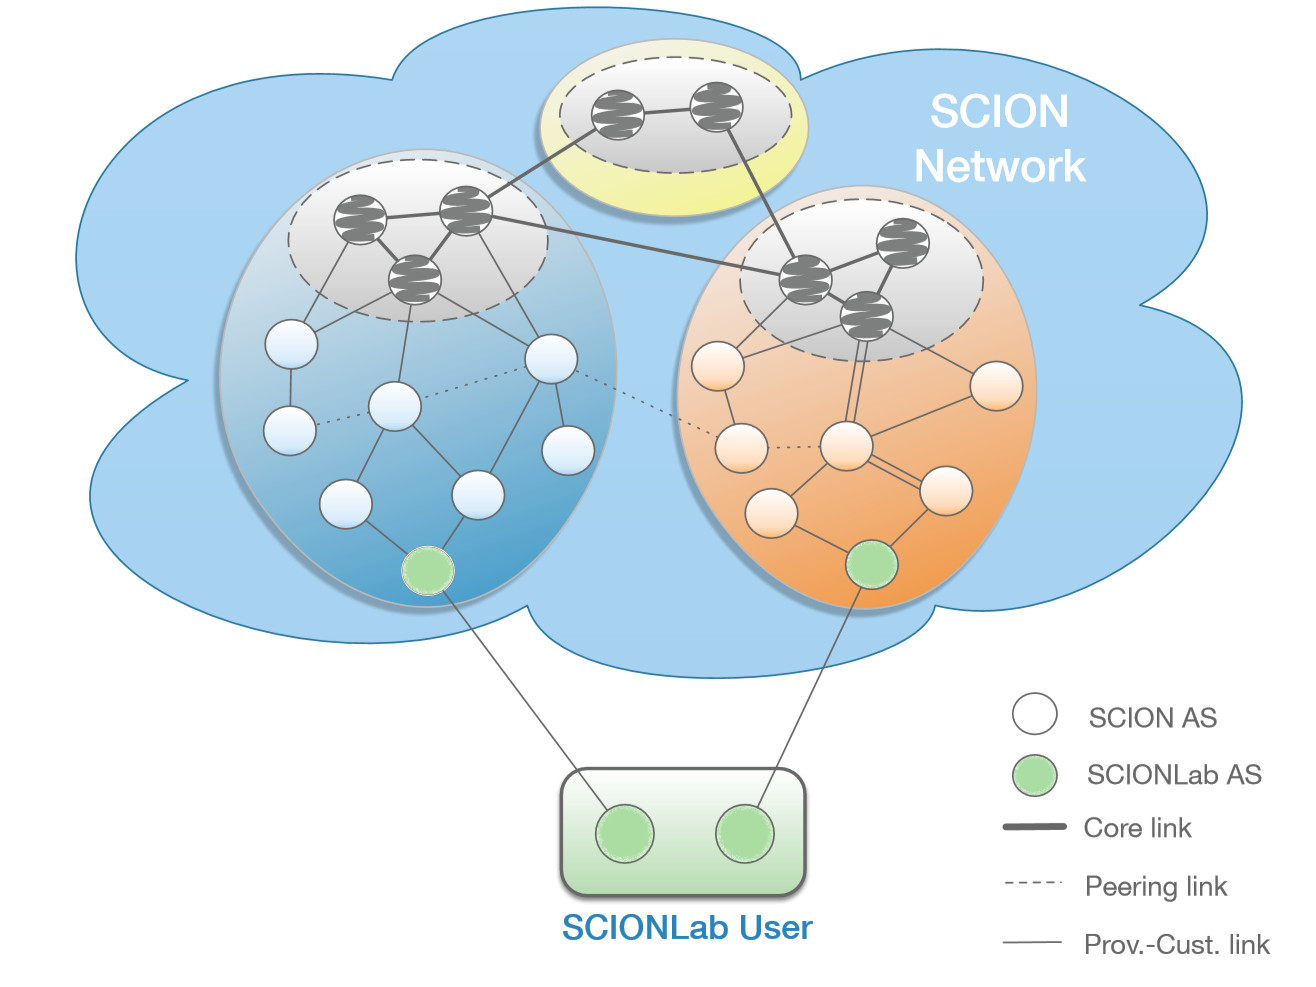
\includegraphics[width=\linewidth]{scionlab.png}}
	\captionof{figure}{An envisioned SCIONLab  testbed environment \cite{scion_book}}
	\label{scionlab_figure}
\end{figure}